
%(BEGIN_QUESTION)
% Copyright 2006, Tony R. Kuphaldt, released under the Creative Commons Attribution License (v 1.0)
% This means you may do almost anything with this work of mine, so long as you give me proper credit

Electrical conductivity in metals is a function of free electrons.  That is to say, free electrons are the {\it charge carriers} for electricity in metallic substances.

Electrical conductivity in semiconductors is a function of either conduction-band electrons or valence-band holes.  Pentavalent dopants add electrons at an energy level just beneath the conduction band of a semiconductor crystal, allowing ambient thermal energy to boost those electrons into the conduction band and serve as charge carriers like free electrons in metals.  This makes an {\it N-type} semiconductor:

$$\includegraphics[width=15.5cm]{i00603x01.eps}$$

Trivalent dopants add ``vacancies,'' or ``holes,'' for valence-band electrons to leap in to with the help of ambient thermal energy.  This makes room for motion of electrons within the valence band, and we call the resulting substance a {\it P-type} semiconductor:

$$\includegraphics[width=15.5cm]{i00603x02.eps}$$

To differentiate the valence-band electron motion in P-type semiconductors from the conduction-band electron motion in N-type semiconductors, we commonly refer to the valence-band electrons' motion in terms of the ``holes'' they leave behind, and treat these holes as positive charge carriers.

\vskip 10pt

Conduction within liquids is another thing entirely.  Since the molecules are free to move about within liquids (and not within solids), entire molecules may act as electrical charge carriers if they are {\it ionized}.  Explain what ``ionization'' is, and distinguish between {\it anions} and {\it cations}.

\underbar{file i00603}
%(END_QUESTION)





%(BEGIN_ANSWER)

An {\it ion} is any atom or molecule that is electrically imbalanced; i.e., its total number of electrons do not equal its total number of protons.

%(END_ANSWER)





%(BEGIN_NOTES)

{\it Anions} are those ions attracted to the positive (anode) terminal in an electrochemical cell.  {\it Cations} are those ions attracted to the negative (cathode) terminal in an electrochemical cell.

%INDEX% Chemistry, ion: anion (defined)
%INDEX% Chemistry, ion: cation (defined)
%INDEX% Measurement, analytical: conductivity

%(END_NOTES)


